\documentclass[a4paper,12pt]{article} 
\usepackage[T2A]{fontenc}			
\usepackage[utf8]{inputenc}			
\usepackage[english,russian]{babel}	
\usepackage{amsmath,amsfonts,amssymb,amsthm,mathtools} 
\usepackage[colorlinks, linkcolor = blue]{hyperref}
\usepackage{upgreek}\usepackage[left=2cm,right=2cm,top=2cm,bottom=3cm,bindingoffset=0cm]{geometry}
\usepackage{graphicx}
\usepackage{subfig}
\usepackage{xcolor}
\author{Дорогинин Д.В.}
\title{3.6.1. Спектральный анализ электрических сигналов.}
\date{}
\begin{document}
\maketitle
\textbf{Цель работы}: 
исследование спектра колебаний электрических сигналов.


\textbf{В работе используются}: генератор сигналов произвольной формы, цифровой осциллограф с функцией быстрого преобразования Фурье.
\section*{Теория}
\subsection*{Разложение сложных сигналов на периодические колебания}
Используется разложение в сумму синусов и косинусов с различными аргументами или, как чаще его называют, \textit{разложение в ряд Фурье}.

Пусть задана функция $f(t)$, которая периодически повторяется с частотой $\Omega_1 = \dfrac{2\pi}{T}$, где $T$ --- период повторения импульсов. Её разложение в ряд Фурье имеет вид 
\begin{equation}
f(t) = \dfrac{a_0}{2} + \sum\limits_{n = 1}^{\infty}\left[a_n \cos \left(n \Omega_1t\right) + b_n \sin \left(n \Omega_1t\right)\right]
\end{equation}
или
\begin{equation}
f(t) = \dfrac{a_0}{2} + \sum\limits_{n = 1}^{\infty}A_n \cos \left(n\Omega_1t-\psi_n\right).
\end{equation}
Если сигнал чётен относительно $t=0$, в тригонометрической записи остаются только члены с косинусами. Для нечетной наоборот.

Коэффициенты определяются по формуле
\begin{equation}
\begin{array}{c}
a_n  = \dfrac{2}{T}\int\limits_{t_1}^{t_1+T}f(t)\cos\left(n \Omega_1 t\right) dt,\\
\\
b_n = \dfrac{2}{T}\int\limits_{t_1}^{t_1+T}f(t)\sin\left(n \Omega_1 t\right) dt.
\end{array}
\end{equation}
Здесь $t_1$ --- время, с которого мы начинаем отсчет.

Сравнив формулы $(1)$ и $(2)$ можно получить выражения для $A_n$  и $\psi_n$:
\begin{equation}
\begin{array}{l}
A_n = \sqrt{a_n^2+b_n^2},\\
 \psi_n = \arctan \dfrac{b_n}{a_n}.
\end{array}
\end{equation}
\subsection*{Периодическая последовательность прямоугольных импульсов}
\begin{center}
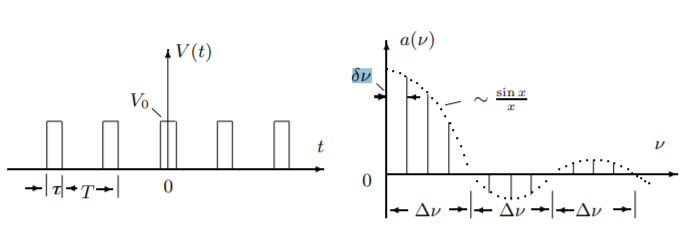
\includegraphics[scale=0.9]{2.png}
\end{center}
Введем величину: $\Omega_1 = \dfrac{2\pi}{T}$,
где $T$ --- период повторения импульсов.

Коэффициенты при косинусных составляющих будут равны
\begin{equation}
a_n = \dfrac{2}{T}\int\limits_{-\tau/2}^{\tau/2}V_0\cos\left(n\Omega_1 t\right)dt = 2V_0\dfrac{\tau}{T}\dfrac{\sin\left(n\Omega_1\tau/2\right)}{n\Omega_1\tau/2} \sim \dfrac{\sin x}{x}.
\end{equation}

Здесь $V_0$ - амплитуда сигнала.

Поскольку наша функция четная, то $b_n = 0$. 

Пусть $T$ кратно $\tau$. Тогда введем ширину спектра, равную $\Delta \omega$ --- расстояние от главного максимума до первого нуля огибающей, возникающего, как нетрудно убедиться при $n = \dfrac{2\pi}{\tau \Omega_1}$. При 
этом
\begin{equation}
\Delta \omega \tau \simeq 2\pi \Rightarrow \Delta \nu \Delta t \simeq 1.
\end{equation}
\subsection*{Периодическая последовательность цугов}
\begin{center}
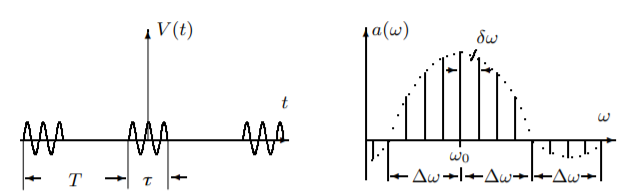
\includegraphics[scale=0.9]{3.png}
\end{center}
Возьмём цуги колебания $V_0 \cos(\omega_0 t)$ с длительностью цуга $\tau$ и периодом повторений $T$.\\
Функция $f(t)$ снова является четной относительно $t = 0$. Коэффициент при $n$-ой гармонике согласно формуле $(3)$ равен
\begin{equation}
a_n = \dfrac{2}{T}\int\limits_{-\tau/2}^{\tau/2}V_0 \cos \left(\omega_0t\right) \cdot \cos\left(n \Omega_1t\right)dt = V_0 \dfrac{\tau}{T}\left( \dfrac{\sin\left[\left(\omega_0 - n \Omega_1\right)\dfrac{\tau}{2}\right]}{\left( \omega_0 - n \Omega_1\right) \dfrac{\tau}{2}} + \dfrac{\sin\left[\left(\omega_0 + n \Omega_1\right)\dfrac{\tau}{2}\right]}{\left( \omega_0 + n \Omega_1\right) \dfrac{\tau}{2}}\right).
\end{equation}
Пусть $T$ кратно $\tau$. Тогда спектры последовательности прямоугильных сигналов и цугов аналогичны, но максимумы сдвинуты на $\omega_0$.
\subsection*{Амплитудно-модулированные колебания}
\begin{center}
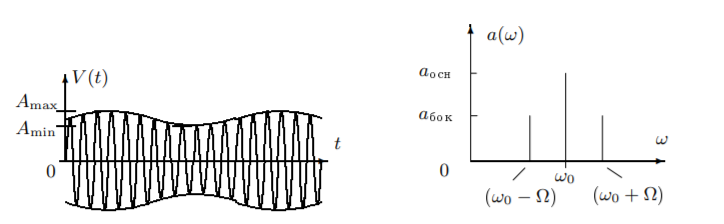
\includegraphics[scale=0.9]{4.png}
\end{center}
Рассмотрим гармонические колебания высокой частоты $\omega_0$, амплитуда которых медленно меняется по гармоническому закону с частотой $\Omega \ll \omega_0$.
\begin{equation}
f(t) = A_0 \left[1+m\cos \Omega t\right] \cos \omega_0 t.
\end{equation}
Коэффициент $m$ называется \textit{глубиной модуляции}. При $m < 1$ амплитуда меняется от минимальной $A_{min} = A_0(1-m)$ до максимальной $A_{max} = A_0(1+m)$. Глубина модуляции может быть представлена в виде
\begin{equation}
m = \dfrac{A_{max}-A_{min}}{A_{max}+A_{min}}.
\end{equation}
Простым тригонометрическим преобразованием уравнения $(8)$ можно найти спектр колебаний
\begin{equation}
f(t) = A_0 \cos \omega_0t + \dfrac{A_0m}{2} \cos \left(\omega_0 + \Omega\right)t + \dfrac{A_0m}{2}\cos\left(\omega_0 - \Omega\right)t.
\end{equation}
\section*{Ход работы}
 \subsection*{Исследование спектра периодических последовательностей прямоугольных импульсов}
Устанавливаем прямоугольные колебания c $\nu_{\text{повт}} = 1$ кГц (период $T = 1$ мс) и длительностью импульса $\tau = T/20 = 50$ мкс.

Получаем на экране спектр сигнала и, изменяя либо $\tau$, либо $\nu_{\text{повт}}$, наблюдаем, как изменяется спектр.
\begin{figure}
    \centering
    \subfloat[$\nu_{\text{повт}} = 1$ кГц, $\tau = 50$ мкс.]{{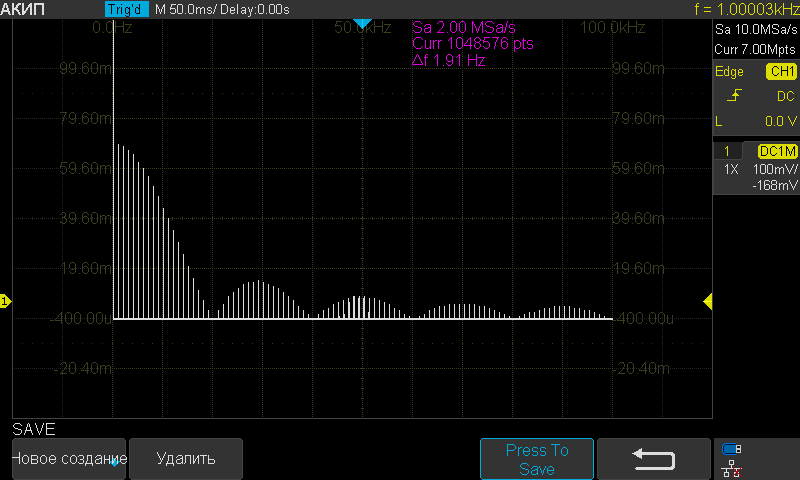
\includegraphics[width=0.5\textwidth]{AKIP0001.png}}}
    \subfloat[$\nu_{\text{повт}} = 1.5$ кГц, $\tau = 50$ мкс.]{{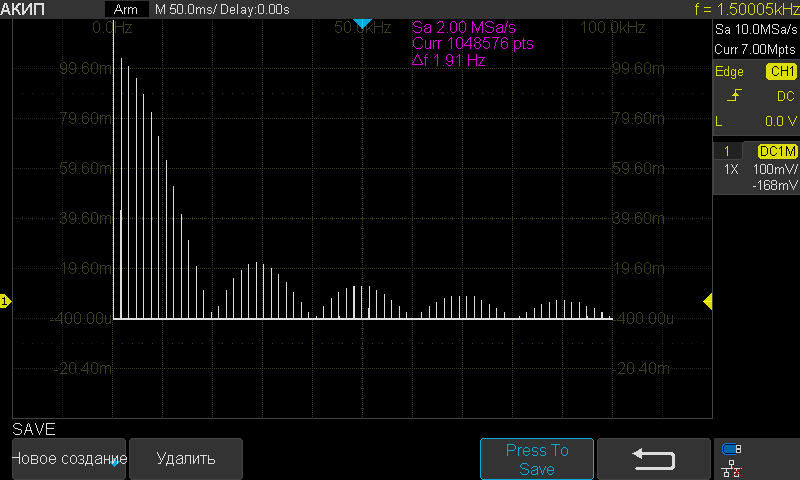
\includegraphics[width=0.5\textwidth]{AKIP0002.png}}}\\
    \subfloat[$\nu_{\text{повт}} = 2$ кГц, $\tau = 50$ мкс.]{{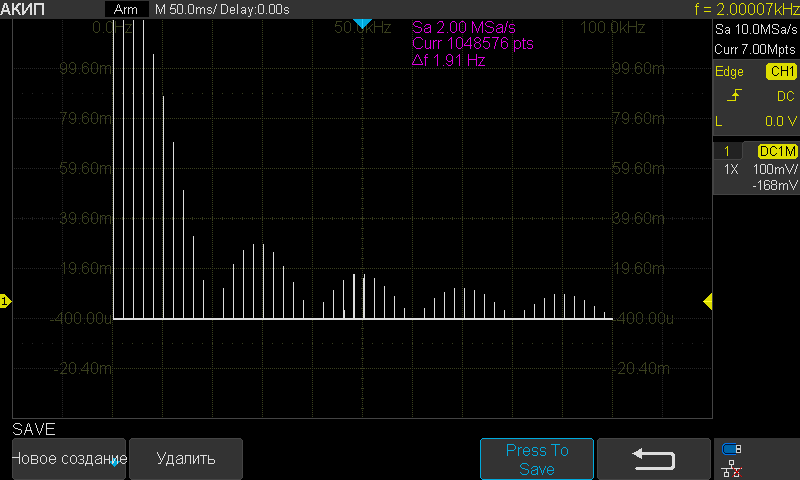
\includegraphics[width=0.5\textwidth]{AKIP0003.png}}}
    \subfloat[$\nu_{\text{повт}} = 2.5$ кГц, $\tau = 50$ мкс.]{{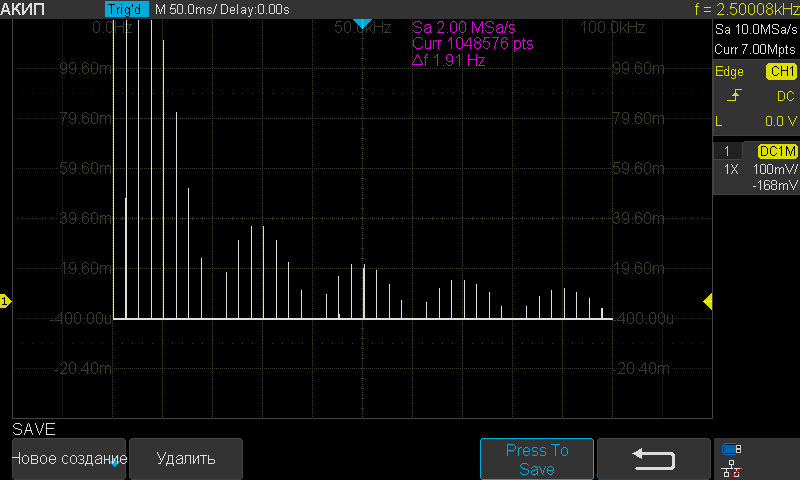
\includegraphics[width=0.5\textwidth]{AKIP0004.png}}}\\
    \subfloat[$\nu_{\text{повт}} = 1$ кГц, $\tau = 60$ мкс.]{{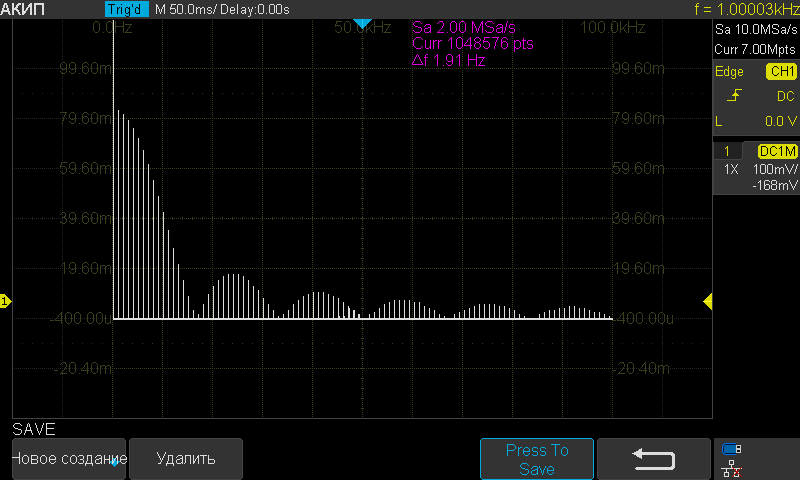
\includegraphics[width=0.5\textwidth]{AKIP0005.png}}}
    \subfloat[$\nu_{\text{повт}} = 1$ кГц, $\tau = 100$ мкс.]{{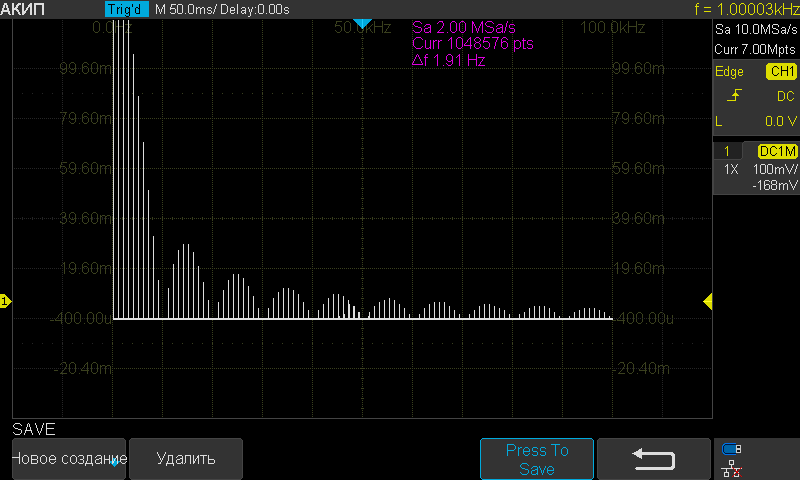
\includegraphics[width=0.5\textwidth]{AKIP0006.png}}}\\
    \subfloat[$\nu_{\text{повт}} = 1$ кГц, $\tau = 150$ мкс.]{{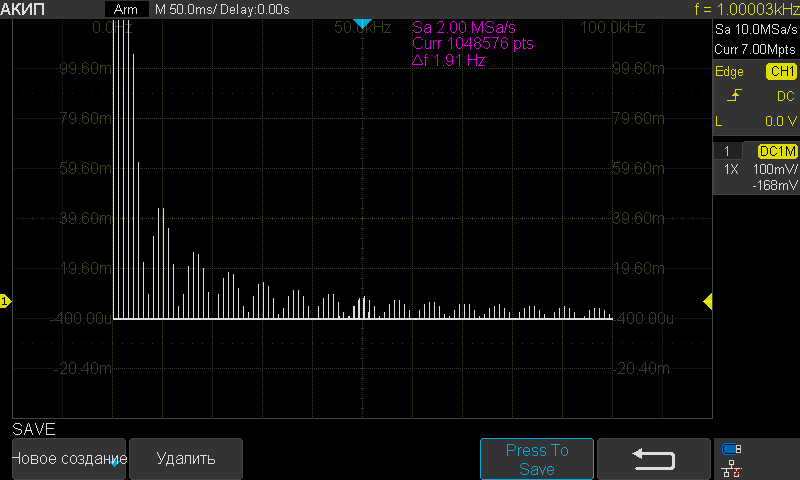
\includegraphics[width=0.5\textwidth]{AKIP0007.png}}}
\end{figure}

Теперь зафиксируем $\nu_{\text{повт}} = 1$ кГц и $\tau = 50$ мкс. Для этих параметров измерим величину $a_n$ и $\nu_n$ для первых 5 гармоник и сравним с рассчитанными значениями по формуле $(5)$.

Теперь проведем измерения зависимости ширины спектра от $\Delta \nu$ и установим зависимость между $\Delta \nu$ и $\tau$, полученную из формулы $(6)$.
\begin{center}
\begin{tabular}{|c|c|c|c|c|c|c|c|}
\hline
$\tau$, мкс & 50 & 75 & 100 & 125 & 150 & 175 & 200 \\ \hline
$\Delta \nu$, кГц & 19.6 & 13.4 & 9.8 & 8.0 & 6.5 & 5.5 & 4.5 \\ \hline
$1/\tau \cdot 10^3$, с$^{-1}$ & 20 & 13 & 10 & 8 & 7 & 6 & 5 \\ \hline
\end{tabular}
\end{center}
\begin{center}
\fbox{$\Delta \nu \tau \approx 1.000 \pm 0.018$}
\end{center}
В итоге получаем, что формула $(6)$ довольно точно выполняется.
\newpage
\subsection*{Исследование спектра периодической последовательности цугов}
Получаем на экране последовательность цугов с характерными параметрами: $\nu_0 = 50$ кГц, $T = 1$ мс, число периодов в одном импульсе $N = 5$ (длительность импульса $\tau = T/\nu_0 = 100$ мкс).
\begin{figure}[h]
    \centering
    \subfloat[Последовательность цугов.]{{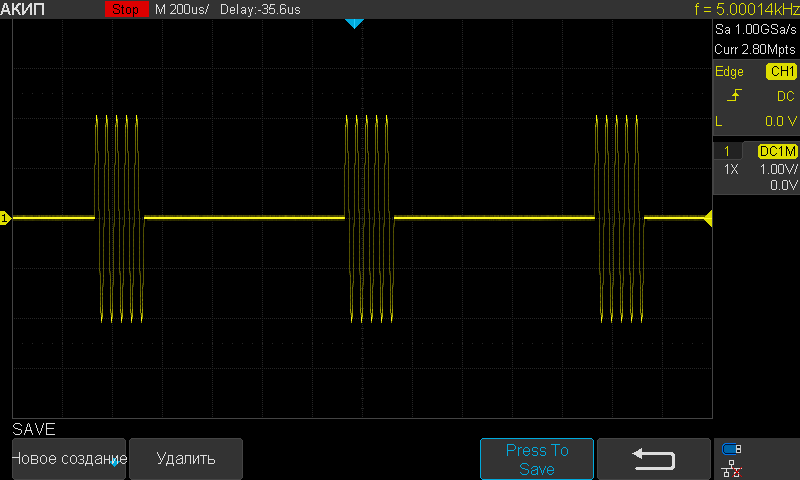
\includegraphics[width=0.5\textwidth]{AKIP0008.png}}}
    \subfloat[Спектр для цугов.]{{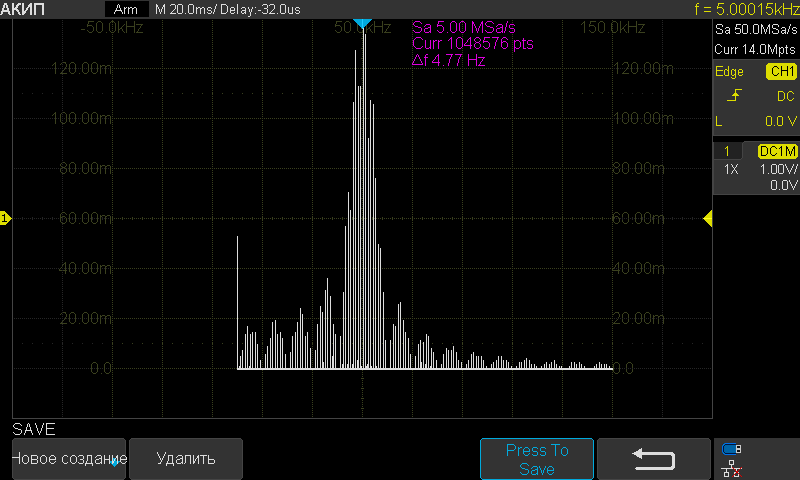
\includegraphics[width=0.5\textwidth]{AKIP0009.png}}}
\end{figure}\\
Теперь будем менять эти параметры по одному и зафиксируем несколько таких изменений:
\begin{figure}[h]
    \centering
    \subfloat[$\nu_0 = 50$ кГц, $T = 1$ мс, $N = 10$.]{{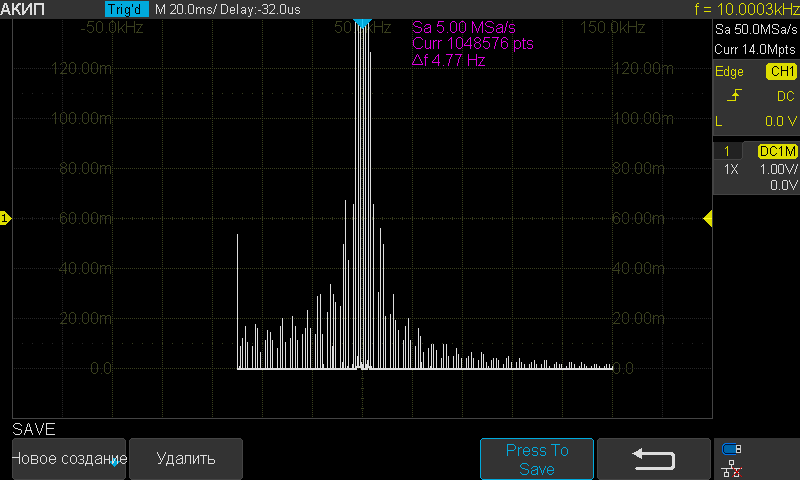
\includegraphics[width=0.5\textwidth]{AKIP0010.png}}}
    \subfloat[$\nu_0 = 50$ кГц, $T = 1$ мс, $N = 15$.]{{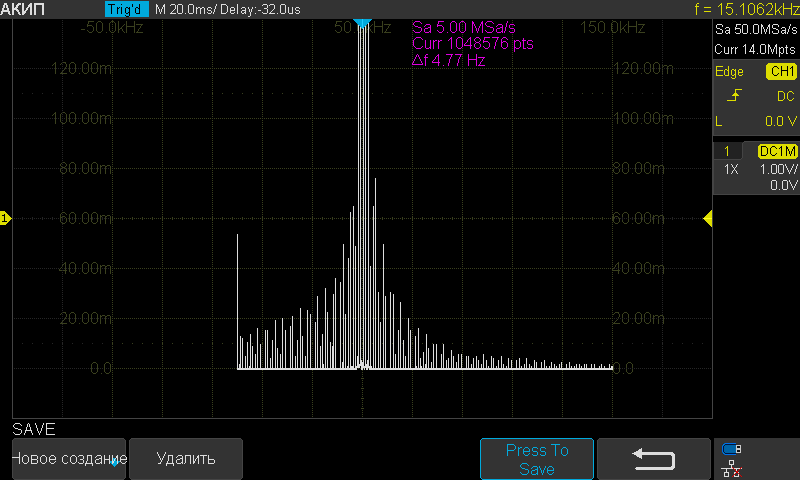
\includegraphics[width=0.5\textwidth]{AKIP0011.png}}}\\
    \subfloat[$\nu_0 = 50$ кГц, $T = 2.5$ мс, $N = 5$.]{{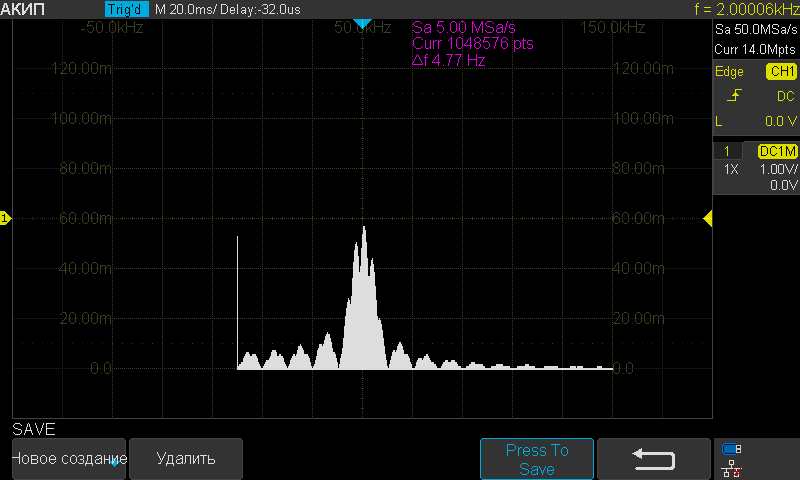
\includegraphics[width=0.5\textwidth]{AKIP0013.png}}}
    \subfloat[$\nu_0 = 50$ кГц, $T = 5$ мс, $N = 5$.]{{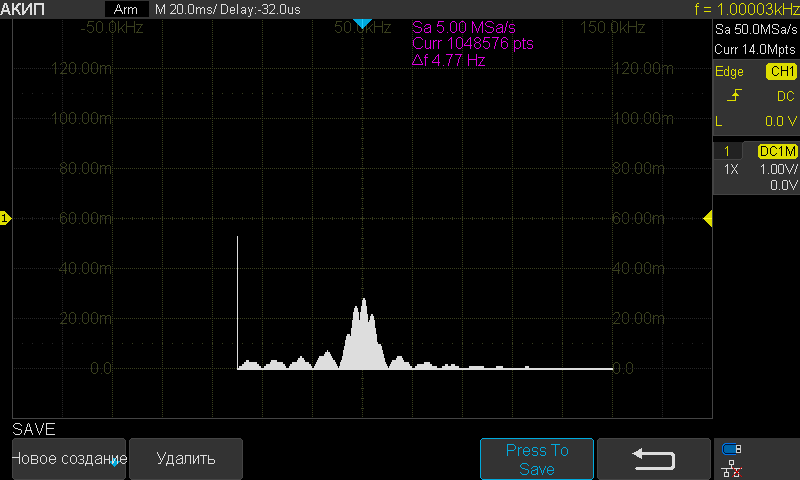
\includegraphics[width=0.5\textwidth]{AKIP0012.png}}}\\
\end{figure}\\
\begin{figure}[h]
    \centering
    \subfloat[$\nu_0 = 75$ кГц, $T = 1$ мс, $N = 5$.]{{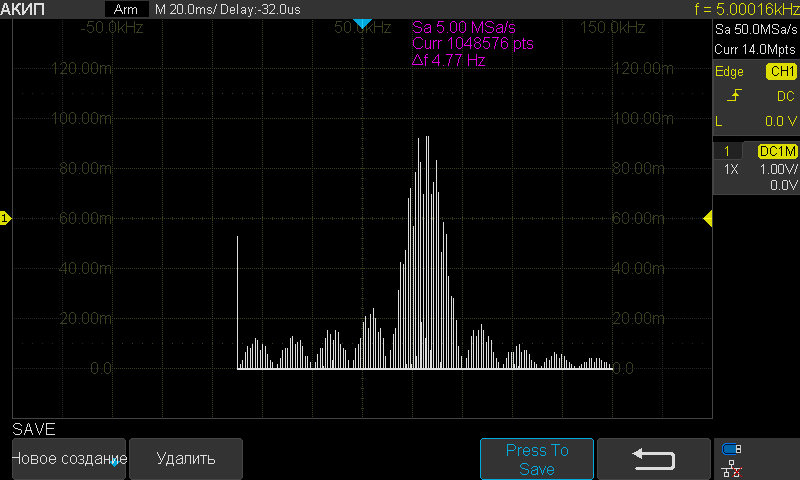
\includegraphics[width=0.5\textwidth]{AKIP0015.png}}}
    \subfloat[$\nu_0 = 100$ кГц, $T = 1$ мс, $N = 5$.]{{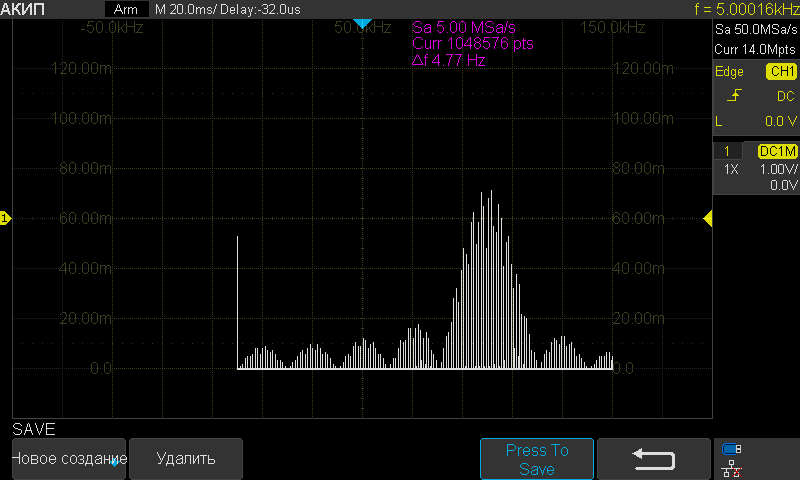
\includegraphics[width=0.5\textwidth]{AKIP0014.png}}}\\
\end{figure}\\

Теперь зафиксируем $\nu_0 = 50$ кГц, $N = 5$. Для этих параметров измерим, меняя $T$ ($\nu_{\text{повт}})$, зависимость $\delta \nu$ от $\tau$. 
\begin{table}[h]
\centering
\begin{tabular}{|c|c|c|c|c|c|c|}
\hline
$\Delta \nu$, кГц       & 23 & 32 & 35 & 38 & 35 & 45 \\ \hline
$n$                                                   & 42 & 33 & 18 & 13 & 10 &  8 \\ \hline
$\nu_{\text{повт}}$, кГц & 0.5 & 1.0  & 2.0  & 3.0  & 4.0 & 6.0  \\ \hline
\end{tabular}
\end{table}\\
Итоговое отношение:
\fbox{$\dfrac{\delta \nu}{\nu_{\text{повт}}} = 1.05 \pm 0.08$}
\subsection*{Исследование спектра амплитудно модулированного сигнала}
Выведем на экран картину амплитудно-модулированного сигнала с характерными параметрами: несущая частота $\nu_0 = 50$ кГц, $\nu_{\text{мод}} = 2$ кГц, глубина модуляции - 50 \% ($m = 0.5$). Картины данного сигнала и его спектра будут выглядеть следующим образом:
\begin{figure}[h]
\centering
 \subfloat[Амплитудно-модулированный сигнал.]{{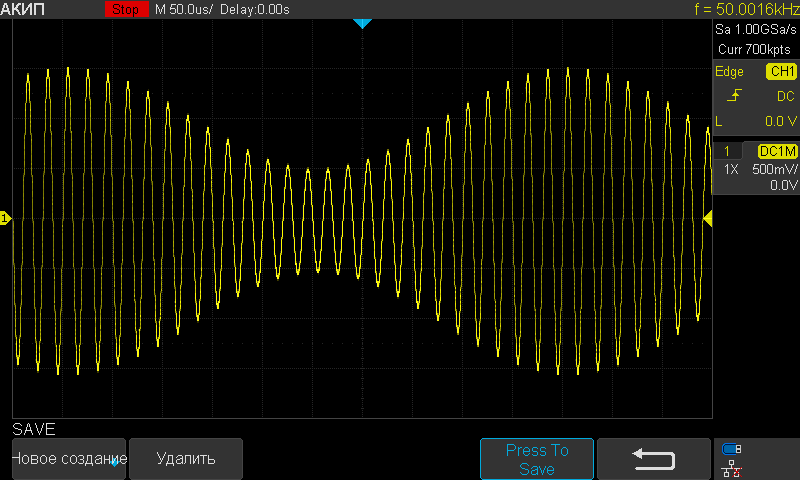
\includegraphics[width = 0.5\textwidth]{AKIP0016.png}}}
    \subfloat[Спектр для $\nu_0 = 50$ кГц, $\nu_{\text{мод}} = 2$ кГц.]{{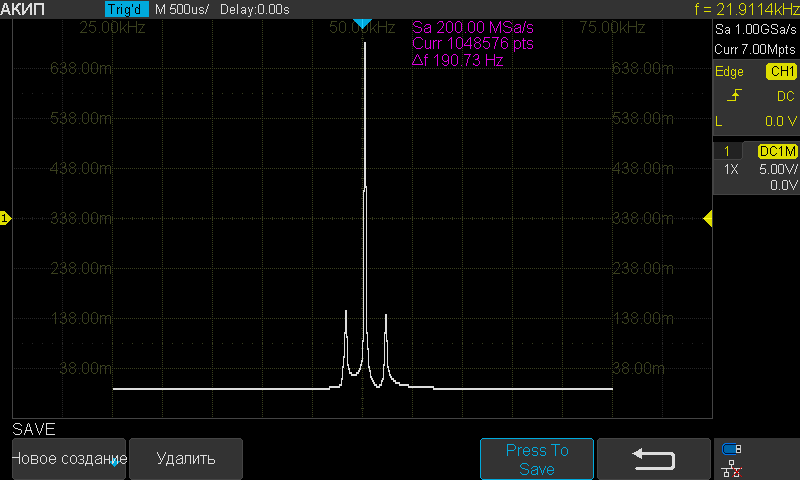
\includegraphics[width=0.5\textwidth]{AKIP0018.png}}}
\end{figure}\\
Найдем для него $A_{max}$ и $A_{min}$ и проверим справедливость формулы $(9)$.
\begin{center}
\begin{tabular}{|c|c|}
\hline
$A_{max}$, В & 1.52 \\ \hline
$A_{min}$, В & 0.48 \\ \hline
$m$ & 0.52 \\ \hline
\end{tabular}
\end{center}
Поскольку мы установили глубину модуляции на $0.5$, а из теории у нас получилась $0.52$, то мы видим, что формула $(9)$ верна.

Получим на экране спектр и будем изменять параметры сигнала:
\begin{figure}[h]
    \centering
    \subfloat[$\nu_0 = 60$ кГц, $\nu_{\text{мод}} = 2$ кГц.]{{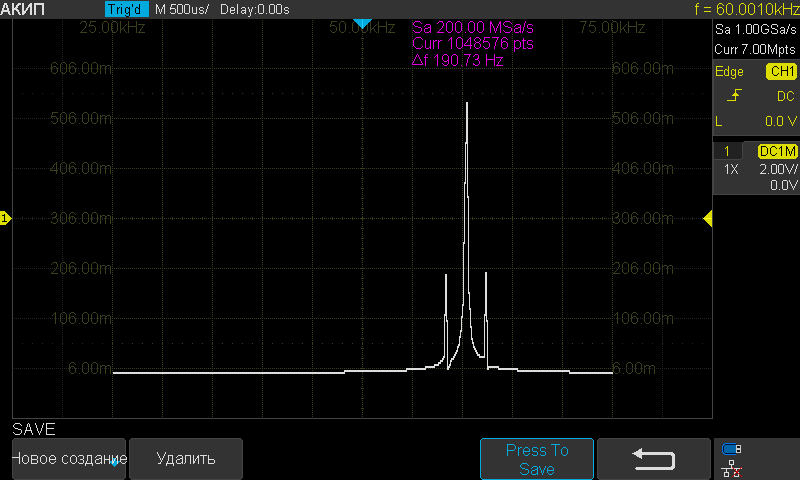
\includegraphics[width=0.5\textwidth]{AKIP0019.png}}}
    \subfloat[$\nu_0 = 70$ кГц, $\nu_{\text{мод}} = 2$ кГц.]{{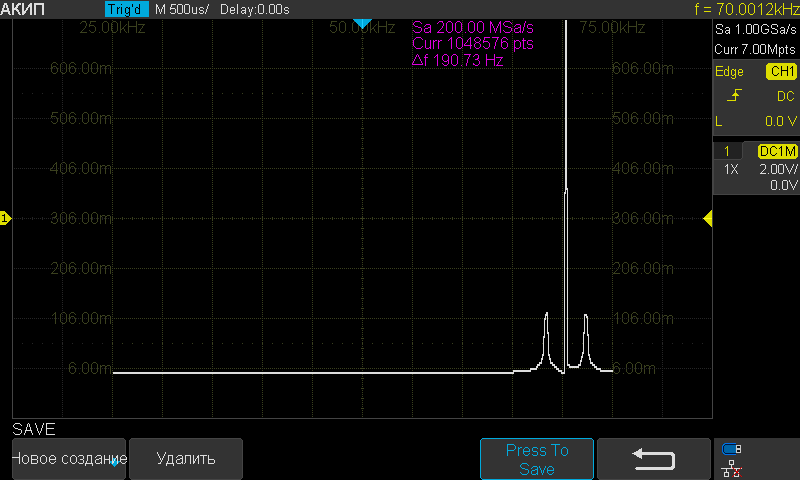
\includegraphics[width=0.5\textwidth]{AKIP0020.png}}}\\
    \subfloat[$\nu_0 = 50$ кГц, $\nu_{\text{мод}} = 8$ кГц.]{{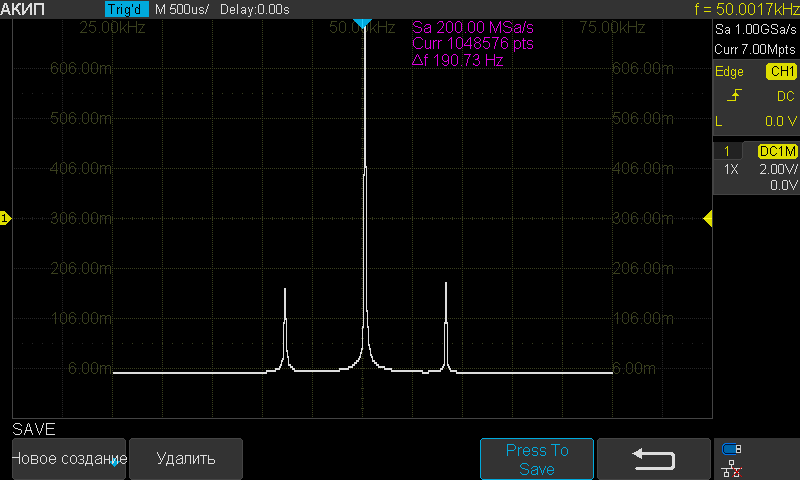
\includegraphics[width=0.5\textwidth]{AKIP0021.png}}}    			\subfloat[$\nu_0 = 50$ кГц, $\nu_{\text{мод}} = 16$ кГц.]{{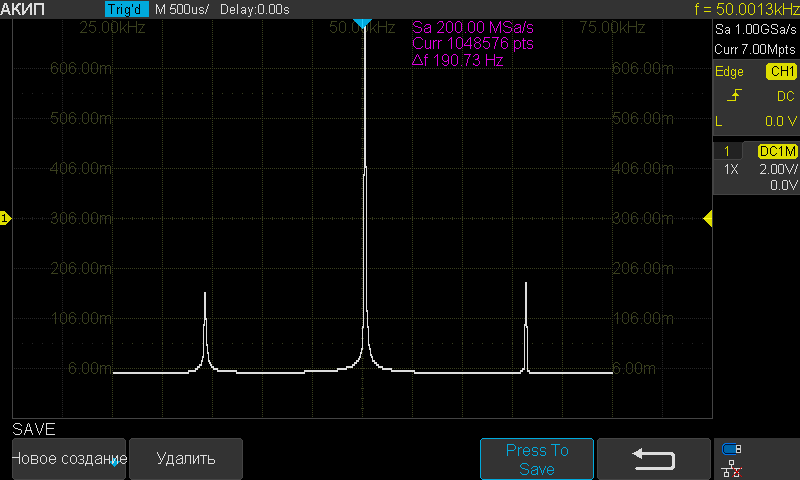
\includegraphics[width=0.5\textwidth]{AKIP0022.png}}}
\end{figure}\\
Из формулы $(10)$ следует, что $a_{\text{осн}} = A_0$, а $a_{\text{бок}} = \dfrac{mA_0}{2}$.
\begin{center}
\begin{tabular}{|c|c|c|c|c|c|}
\hline
$m$, \% & 10 & 25 & 50 & 75 & 100 \\ \hline
$a_{\text{бок}}$, мВ & 360 & 820 & 1660 & 2320 & 3260 \\ \hline
$a_{\text{осн}}$, мВ & 6240 & 6240 & 6240 & 6240 & 6240 \\ \hline
$a_{\text{бок}}/a_{\text{осн}}$ & 0.06 & 0.13 & 0.27 & 0.37 & 0.52 \\ \hline
$a_{\text{бок}}/a_{\text{осн}} \cdot m$, \% & 57.7 & 52.6 & 53.2 & 49.6 & 52.2 \\ \hline
\multicolumn{6}{|c|}{$a_{\text{бок}}/a_{\text{осн}} \cdot m = (53.1 \pm 1.3)$\%} \\ \hline
\end{tabular}
\end{center}
Из $(10)$ имеем $\dfrac{a_{\text{бок}}}{a_{\text{осн}}} \cdot m = 0.5$, что с высокой точностью повторяет наш результат.
\end{document}